%%%%%%%%%%%%%%%%%%%%%%%%%%%%%%%%%%%%%%%%%
% Large Colored Title Article
% LaTeX Template
% Version 1.1 (25/11/12)
%
% This template has been downloaded from:
% http://www.LaTeXTemplates.com
%
% Original author:
% Frits Wenneker (http://www.howtotex.com)
%
% License:
% CC BY-NC-SA 3.0 (http://creativecommons.org/licenses/by-nc-sa/3.0/)
%
%%%%%%%%%%%%%%%%%%%%%%%%%%%%%%%%%%%%%%%%%

%----------------------------------------------------------------------------------------
%	PACKAGES AND OTHER DOCUMENT CONFIGURATIONS
%----------------------------------------------------------------------------------------

\documentclass[DIV=calc, paper=a4, fontsize=11pt, twocolumn]{article}	 % A4 paper and 11pt font size

\usepackage{courier} % enables code-like styles
\usepackage{graphicx} % enables importing images
\usepackage[cm]{fullpage} % page margin fix
\usepackage{lipsum} % Used for inserting dummy 'Lorem ipsum' text into the template - will be removed in final version
\usepackage[english]{babel} % English language/hyphenation
\usepackage[protrusion=true,expansion=true]{microtype} % Better typography
\usepackage{amsmath,amsfonts,amsthm} % Math packages
\usepackage[svgnames]{xcolor} % Enabling colors by their 'svgnames'
\usepackage[hang, small,labelfont=bf,up,textfont=it,up]{caption} % Custom captions under/above floats in tables or figures
\usepackage{booktabs} % Horizontal rules in tables
\usepackage{fix-cm}	 % Custom font sizes - used for the initial letter in the document

\usepackage{sectsty} % Enables custom section titles
\usepackage{titlesec} % enables inserting margins around sections and subsections

\allsectionsfont{\usefont{OT1}{phv}{b}{n}} % Change the font of all section commands

\usepackage{pgfplots} % package to plot graphs using data
\usepackage{fancyhdr} % Needed to define custom headers/footers
\pagestyle{fancy} % Enables the custom headers/footers
\usepackage{lastpage} % Used to determine the number of pages in the document (for "Page X of Total")

% Headers
% raisebox moves text in header up, header text needs to be enclosed in curly brackets
\lhead{\raisebox{0.5\height} {COMS30115 - Computer Graphics}}
\chead{}
\rhead{\raisebox{0.5\height} {jh13290, mm13354}}

% Footers
\lfoot{}
\cfoot{}
\rfoot{\footnotesize Page \thepage\ of \pageref{LastPage}} % "Page 1 of 2"

\renewcommand{\headrulewidth}{0.2pt} % Thin header rule
\renewcommand{\footrulewidth}{0.4pt} % Thin footer rule
\headsep 5pt
\usepackage{lettrine} % Package to accentuate the first letter of the text
\newcommand{\initial}[1]{ % Defines the command and style for the first letter
	\lettrine[lines=3,lhang=0.3,nindent=0em]{
		\color{Goldenrod}
		{\textsf{#1}}}{}}

\setlength{\intextsep}{2pt}
\setlength{\textfloatsep}{2pt}
%----------------------------------------------------------------------------------------
%	TITLE SECTION
%----------------------------------------------------------------------------------------

\usepackage{titling} % Allows custom title configuration

\newcommand{\HorRule}{\color{Goldenrod} \rule{\linewidth}{1pt}} % Defines the blue horizontal rule under the title
	

\pretitle{\vspace{-10pt} \begin{center} \fontsize{25}{25} \usefont{OT1}{phv}{b}{n} \color{Goldenrod} \selectfont} % Horizontal rule before the title
	
	\title{Rasterizer} % Your article title
	
	\posttitle{\end{center}} % Whitespace under the title

\preauthor{ \begin{center}\large \lineskip -1em \usefont{OT1}{phv}{b}{sl} \color{Goldenrod}} % Author font configuration
	
	\author{Jason Haciepiri, Maria Marinova} % Your name
	
	\postauthor{\vspace{-10pt} \footnotesize \usefont{OT1}{phv}{m}{sl} \color{Black} % Configuration for the institution name
		
		\par\end{center}\HorRule } % Horizontal rule after the title

\date{\vspace{-30pt}} % Add a date here if you would like one to appear underneath the title block

%----------------------------------------------------------------------------------------

\begin{document}
	
	\maketitle % Print the title
	
	\thispagestyle{fancy} % Enabling the custom headers/footers for the first page 
	
	%----------------------------------------------------------------------------------------
	%	INTRODUCTION
	%----------------------------------------------------------------------------------------
	
	% The first character should be within \initial{}
	\initial{R}\textbf{asterization is a way of computing a 2D image representation of a 3D scene. It is faster than raytracing, and hence typically used for real-time visualisation. However, it is not as accurate as raytracing.}
	
	%----------------------------------------------------------------------------------------
	%	ARTICLE CONTENTS
	%----------------------------------------------------------------------------------------
	
	\section*{1. Compiling and running the code}

	The project includes a Makefile, which compiles the code. It contains the -O3 flag in CC\_Opts so that the code is compiled in the most optimised way. The -lX11 flag is added to the linker options LL\_Opts to allow communication with the X11 Windows Manager. The flag -fopenmp is added to the CC flags. The last two flags allow for parallelism in the code, which will be elaborated on in Section 3. 
	\par
	The project is compiled and run using the command: \par
		\texttt{make \&\&  .\textbackslash Build\textbackslash skeleton}
 

	\section*{2. Parts 1 and 2}
	The first aspect implemented was projecting points from 3D to 2D in perspective. As the pinhole camera model is used, the relation is derived using similar triangles; the width and height of the screen are also taken into account.
	\par
	The camera can be moved via the keyboard -- translation and rotation are implemented in the \texttt{Update()} function.
	\par
	The vertices of the triangles which compose the 3D scene are therefore projected to the 2D image. Interpolation is used to draw the edges between them, and hence produce the respective triangles in the 2D image.
	\par
	A depth buffer is implemented to ensure the 2D representation reflects the position of the objects in the 3D scene.
	\par
	The illumination can be computed per vertex or per pixel -- the former is faster but less accurate. It is computed as a combination of direct and indirect light, and is also affected by the objects reflectance. While in the base case the reflectance is simply the colour of the objects, it can be extended to hold the reflectance properties of the materials.
	\par
	In order to simulate illumination, a light source which can be moved via the keyboard is added.
	\begin{figure}[!htp]
		\begin{minipage}{.95\linewidth}
			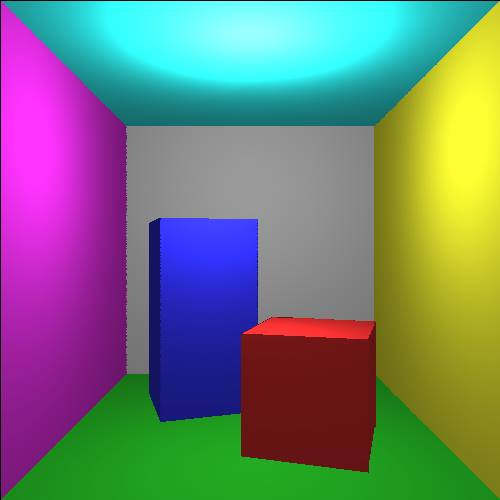
\includegraphics[width=\linewidth]{rast_base.jpg}
			\captionsetup{belowskip=4pt,aboveskip=-11pt}
			\caption{Rasterizer base}
			\label{graph}
		\end{minipage}
	\end{figure}
	
	\section*{3. Extensions}
	Jason does this.

	
\end{document}